\documentclass{beamer}

% There are many different themes available for Beamer. A comprehensive
\usetheme{Frankfurt}

\title{High Performance DSL's in OCaml}

% A subtitle is optional and this may be deleted
\subtitle{Final Year Project - Midterm Evaluation}

\author{Rohit Mukherjee}
% - Give the names in the same order as the appear in the paper.
% - Use the \inst{?} command only if the authors have different
%   affiliation.

\institute[National University of Singapore] % (optional, but mostly needed)

\date{November 27, 2014}

\subject{Computer Engineering}
\pgfdeclareimage[height=0.7cm]{university-logo}{figures/nus_logo}
\logo{\pgfuseimage{university-logo}}

\begin{document}

\begin{frame}
  \titlepage
  {Supervisor: Dr. Chin Wei Ngan}
  \newline{}
  {Project ID: H018570}
\end{frame}

\begin{frame}{Outline}
  \tableofcontents
  % You might wish to add the option [pausesections]
\end{frame}

% Section and subsections will appear in the presentation overview
% and table of contents.
\section{Introduction}

\subsection{Problem}

\begin{frame}{Problem}{Lack of mature frameworks/DSLs for system testing}
  \begin{itemize}
  \item {
    DSLs provide a high-level user-oriented view for software development.
  }
  \item {
    Strongly-typed functional languages, like Scala - great for writing DSLs 
  }
  \item {
  Dearth of mature frameworks and tools available for system testing which can make the process painless and convenient. 
  }
  \item {
  \bf{Existing Frameworks:} Not exactly suitable for system testing
  }
  \end{itemize}
\end{frame}

\begin{frame}{Existing Frameworks}
\begin{figure}[h!]
  \centering
    
\includegraphics[height=50px]{figures/selenium.jpg}
    
\includegraphics[height=50px]{figures/junit-logo.png}
\end{figure}
\begin{figure}[h!]
  \centering
    
\includegraphics[height=100px]{figures/scalaTest.jpg}
    
\includegraphics[height=40px]{figures/cucumber.png}
\end{figure}
\end{frame}


\subsection{Solution}
\begin{frame}{Solution}{A DSL for System Testing}
  \begin{itemize}
  \item {
    In this project, some of the different ways scalable, high - performance DSLs could be written were examined and evaluated.
  }
  \item {
    Focus for this semester was to develop the various types and language of the DSL.
  }
  \item {
  DSL objectives and goals discussed next slide
  }
  \end{itemize}
\end{frame}

\subsection{DSL Requirements}
\begin{frame}{DSL Requirements}
  \begin{itemize}
    \item Testing systems with inputs and matching against specified outputs
    \item Testing whether the system is functional as a whole and generates output
    \item Intuitive, declarative syntax for testers
    \item Ease of debugging and use
    \item Extensibility of the DSL
    \item Ease of integration with application code
  \end{itemize}
\end{frame}

\section{Literature Review}

\subsection{DSL Design}

\begin{frame}{1. Embedded DSLs in Scala}
\begin{block}{DSLs in Action, Ghosh, Manning Publications}
Ghosh discusses two approaches to constructing internal DSLs - \textbf{Embedded} and \textbf{Generative}. Statically typed languages offer types as one of the means to abstract domain semantics and make the surface syntax of the DSL concise. Typed models come with a
guarantee of some level of implicit consistency in the programming model. 
\end{block}
\end{frame}

\begin{frame}{Approaches to DSL Design}
\begin{figure}[h!]
  \centering
    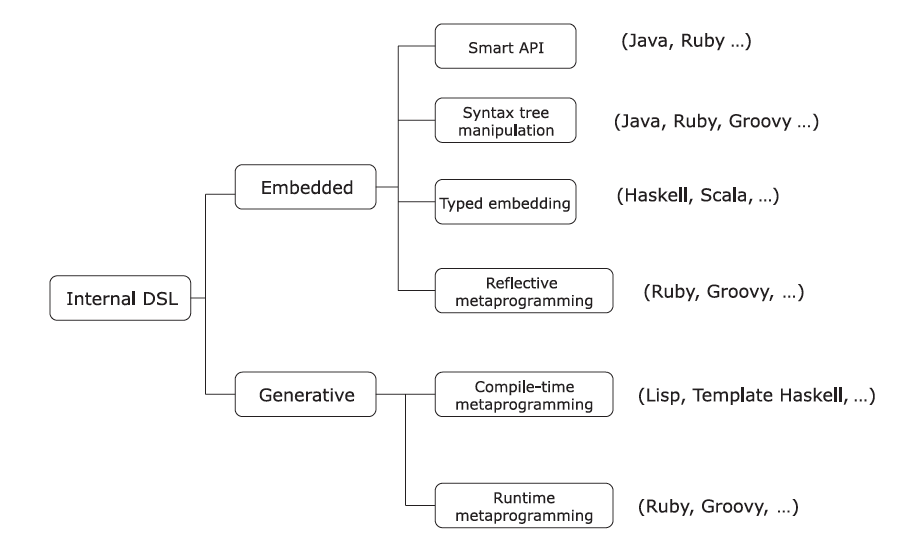
\includegraphics[height=200px]{figures/classification.png}
  \caption{Micro - classification of DSLs}
\end{figure}
\end{frame}

\begin{frame}{A simple JSON DSL}
\begin{figure}[h!]
  \centering
    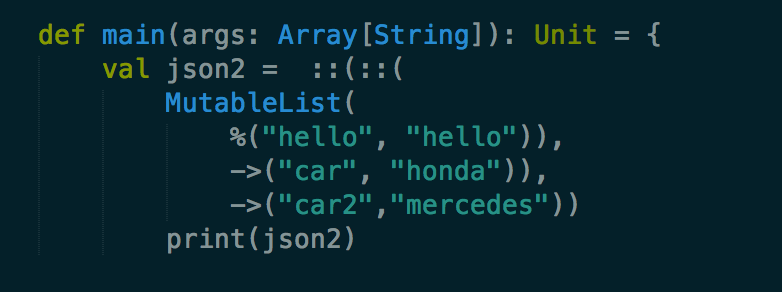
\includegraphics[height=100px]{figures/json.png}
  \caption{JSON DSL using type embedding}
\end{figure}
\textbf{Link:} https://github.com/rohitmukherjee/High-Performance-DSLs
\end{frame}

\begin{frame}{2: Lightweight Modular Staging}
\begin{block}{Lightweight Modular Staging, Rompf \& Odersky}
Rompf and Odersky (2010) talk about an alternative approach to writing DSLs in Scala using a run - time code generation approach called lightweight modular staging. This approach involves both a generative and an embedded approach. The DSL is provided as a library and involves run - time code generation in different stages. The approach is called \textbf{Light - Weight Modular Staging (LMS)}.
\end{block}
\end{frame}

\begin{frame}{LMS}
\begin{figure}[h!]
  \centering
    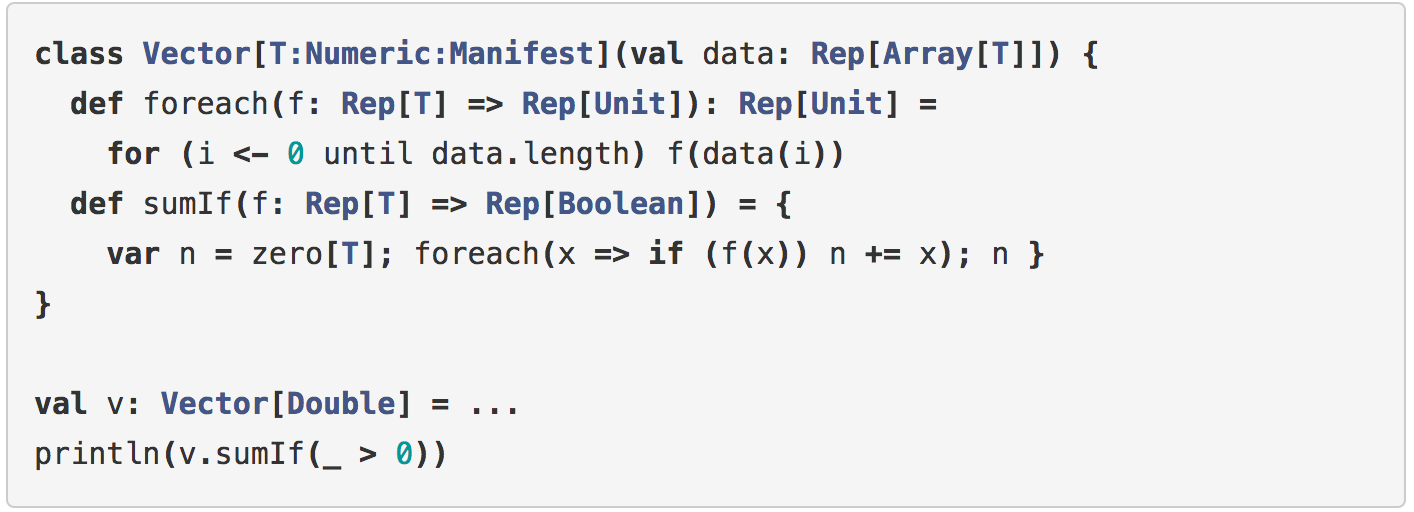
\includegraphics[height=150px]{figures/lms1.png}
  \caption{Code written using LMS}
\end{figure}
\end{frame}

\begin{frame}{LMS}
\begin{figure}[h!]
  \centering
    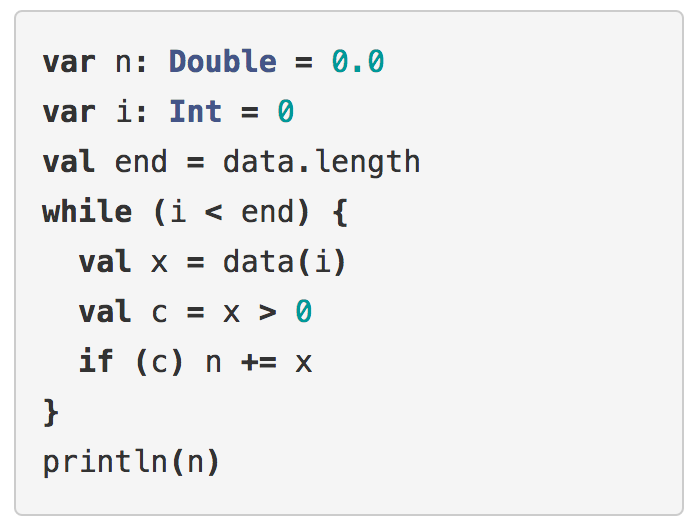
\includegraphics[height=150px]{figures/lms2.png}
  \caption{Code at compile time}
\end{figure}
\end{frame}

\begin{frame}{3: Delite, a framework for high performance DSLs}
\begin{block}{Delite, Odersky}
A third approach to writing embedded, high - performance DSLs conducted by Odersky built upon the concept of using lightweight modular staging. The research resulted in a framework called Delite. Delite's compilation pipeline takes care of optimizing for target hardware such as multi - core processors, GPUs and computing clusters.
\end{block}
\end{frame}
 
\begin{frame}{Delite Compilation Pipeline}
\begin{figure}[h!]
  \centering
    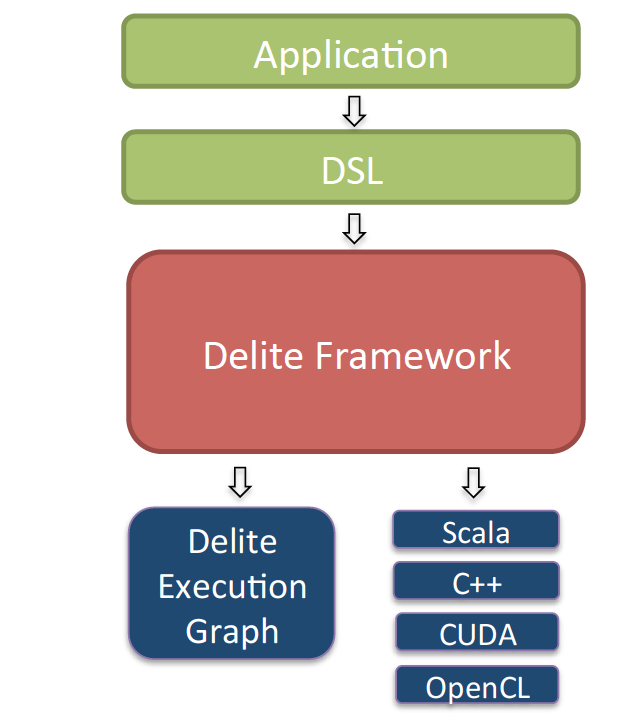
\includegraphics[height=150px]{figures/delite.png}
  \caption{Delite compilation pipeline}
\end{figure}
\end{frame}

\begin{frame}{Approach chosen for this semester}
\begin{itemize}
\item Approach 1 of embedded DSL in Scala was chosen for this semester
\item This was done to understand the various types required and implement functionality
\item Performance optimizations will be considered in the next semester
\end{itemize}
\end{frame}


\section{Progress Report}

\subsection{Overview of Progress}
\begin{frame}{Overview of Progress}
\begin{itemize}
\item Types required to model the domain
\item Basic DSL which can test any system/executable
\item Declarative, natural language like syntax
\end{itemize}
\begin{figure}[h!]
  \centering
    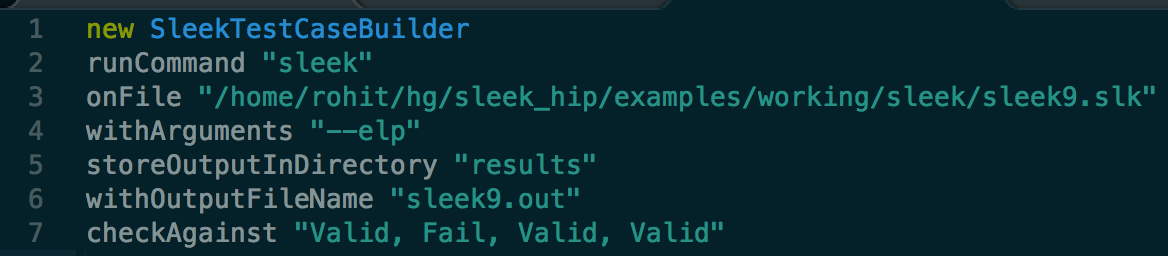
\includegraphics[height=70px]{figures/code_snippet.png}
  \caption{Code Snippet}
\end{figure}
\end{frame}

\subsection{Design Choices}
\begin{frame}{Reasons for making certain design choices}
\begin{itemize}
\item Internal DSL approach
\item Choice of Scala as language of implementation
\item Choice of certain design patterns
\end{itemize}
\begin{figure}[h!]
  \centering
    
\includegraphics[height=50px]{figures/scala_logo.png}
\end{figure}
\end{frame}

\subsection{Functionality Completed}
\begin{frame}{Functionality Completed}
\begin{itemize}
\item Construct test cases for individual systems against expected output
\item Run tests for all test files in a directory against previously generated output
\item Custom matchers based on regex and diff
\item Declarative syntax
\item generate scripts to run test files in a directory
\end{itemize}
\end{frame}


\subsection{Thoughts on preliminary investigation}
\begin{frame}{Thoughts on investigation}
The following conclusions were drawn from the initial investigation:
\begin{itemize}
\item Scala provides a friendly ecosystem to write DSLs in many ways (as discussed)
\item System Testing is a domain which requires more tooling/frameworks
\item Ongoing research to optimize Scala for DSLs
\item Design Patterns yield clean, reusable syntax and API
\end{itemize}
\end{frame}

\section{Research Plan}

\begin{frame}{Research Plan}
\begin{itemize}
\item Complete DSL feature list
\item Features to provide greater automation/unit testing
\item Lower level optimizations, revisit Delite and LMS
\item Extend DSL to include performance testing
\item Make DSL easy to use with real projects
\end{itemize}
\end{frame}

\begin{frame}{Research Plan}
\begin{figure}[h!]
  \centering
    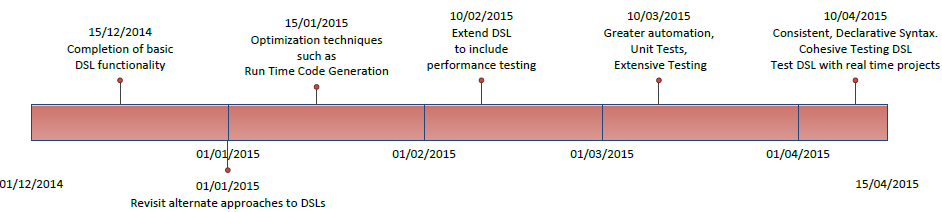
\includegraphics[width=333px]{figures/timeline.png}
\end{figure}
\end{frame}

\section*{Summary}

\begin{frame}{Summary \& QA}
  \begin{itemize}
  \item
     \alert{DSL for system testing} using Scala.
  \item
     Aim to make it an \alert{extensible system testing DSL}
  \item
     Provide high performance through \alert{LMS/Delite like optimizations} in the next semester.
  \end{itemize}
\end{frame}

\end{document}


